\ifx\allfiles\undefined
\documentclass[12pt, a4paper, oneside, UTF8]{ctexbook} 
\usepackage{amsmath}   % 数学公式
\usepackage[dvipsnames]{xcolor}
\usepackage{amsthm}    % 定理环境
\usepackage{amssymb}   % 更多公式符号
\usepackage{graphicx}  % 插图
\usepackage{mathrsfs}  % 数学字体
\usepackage{enumitem}  % 列表
\usepackage{geometry}  % 页面调整
\usepackage{unicode-math}
\usepackage{extarrows}
\usepackage{subfigure}
\usepackage{extarrows}
\usepackage{footnote}
\usepackage{svg}
\usepackage[colorlinks,linkcolor=black]{hyperref}
\usepackage{supertabular}
\usepackage{tcolorbox}
\usepackage{ulem}
\usepackage{framed}
\usepackage{float}
\usepackage{microtype}
\newcommand{\arccot}{\mathrm{arccot}\,}
\tcbuselibrary{breakable}
\tcbuselibrary{most}
\newcounter{problemname}
\newenvironment{solution}{\par\noindent\textbf{解答. }}{\par}
\newenvironment{note}{\par\noindent\textbf{题目\arabic{problemname}的注记. }}{\par}
\definecolor{shadecolor}{RGB}{241, 241, 255}
\newenvironment{problem}{\begin{shaded}\stepcounter{problemname}\par\noindent\textbf{题目\arabic{problemname}. }}{\end{shaded}\par}

\graphicspath{ {figure/},{../figure/}, {config/}, {../config/} }  % 配置图形文件检索目录
\linespread{1.2} % 行高

% 页码设置
\geometry{top=25.4mm,bottom=25.4mm,left=20mm,right=20mm,headheight=2.17cm,headsep=4mm,footskip=12mm}

% 设置列表环境的上下间距
\setenumerate[1]{itemsep=5pt,partopsep=0pt,parsep=\parskip,topsep=5pt}
\setitemize[1]{itemsep=5pt,partopsep=0pt,parsep=\parskip,topsep=5pt}
\setdescription{itemsep=5pt,partopsep=0pt,parsep=\parskip,topsep=5pt}

% 定理环境
% ########## 定理环境 start ####################################

% #### 将 config.tex 中的定理环境的对应部分替换为如下内容
% 定义单独编号,其他四个共用一个编号计数 这里只列举了五种,其他可类似定义(未定义的使用原来的也可)
\newtcbtheorem[auto counter, number within=section, list type=subsubsection, list inside=toc]{defn}{定义}
{
    colback=green!5,colframe=green!35!black,fonttitle=\bfseries, title={Comment \thetcbcounter}, list entry={Comment \thetcbcounter\quad}, %标题
    breakable, %支持跨页
    before upper={\parindent10pt\noindent},  % 支持缩进。\noindent:首行不缩进
    % left = 2mm, %文字离线框左边的边距
    % right = 1mm,%同上
    % top = 1mm,%同上
    % bottom = 1mm,%同上
    % arc is angular = 1mm, % 棱角线框
    % sharp corners, % 直角线框
    % enhanced,frame hidden, % 隐藏线框
    % enhanced, drop fuzzy shadow,  % 显示阴影
}
{def}

\newtcbtheorem[auto counter, number within=section, list type=subsubsection, list inside=toc]{lemma}{引理}
{
    colback=SeaGreen!10!CornflowerBlue!10,colframe=RoyalPurple!55!Aquamarine!100!,fonttitle=\bfseries, title={Comment \thetcbcounter}, list entry={Comment \thetcbcounter\quad}, %标题
    breakable, %支持跨页
    before upper={\parindent10pt\noindent},  % 支持缩进。\noindent:首行不缩进
    % left = 2mm, %文字离线框左边的边距
    % right = 1mm,%同上
    % top = 1mm,%同上
    % bottom = 1mm,%同上
    % arc is angular = 1mm, % 棱角线框
    % sharp corners, % 直角线框
    % enhanced,frame hidden, % 隐藏线框
    % enhanced, drop fuzzy shadow,  % 显示阴影
}
{lem}


\newtcbtheorem[auto counter, number within=section, list type=subsubsection, list inside=toc]{them}{定理}
{
    colback=Salmon!20, colframe=Salmon!90!Black,fonttitle=\bfseries, title={Comment \thetcbcounter}, list entry={Comment \thetcbcounter\quad}, %标题
    breakable, %支持跨页
    before upper={\parindent10pt\noindent},  % 支持缩进。\noindent:首行不缩进
    % left = 2mm, %文字离线框左边的边距
    % right = 1mm,%同上
    % top = 1mm,%同上
    % bottom = 1mm,%同上
    % arc is angular = 1mm, % 棱角线框
    % sharp corners, % 直角线框
    % enhanced,frame hidden, % 隐藏线框
    % enhanced, drop fuzzy shadow,  % 显示阴影
}
{them}
\newtcbtheorem[auto counter, number within=section, list type=subsubsection, list inside=toc]{criterion}{注}
{
    colback=CornflowerBlue!10,colframe=RoyalPurple!55!Aquamarine!100!,fonttitle=\bfseries, title={Comment \thetcbcounter}, list entry={Comment \thetcbcounter\quad}, %标题
    breakable, %支持跨页
    before upper={\parindent10pt\noindent},  % 支持缩进。\noindent:首行不缩进
    % left = 2mm, %文字离线框左边的边距
    % right = 1mm,%同上
    % top = 1mm,%同上
    % bottom = 1mm,%同上
    % arc is angular = 1mm, % 棱角线框
    % sharp corners, % 直角线框
    % enhanced,frame hidden, % 隐藏线框
    % enhanced, drop fuzzy shadow,  % 显示阴影
}
{cri}

\newtcbtheorem[auto counter, number within=section, list type=subsubsection, list inside=toc]{corollary}{推论}
{
    colback=Emerald!10,colframe=cyan!40!black,fonttitle=\bfseries, title={Comment \thetcbcounter}, list entry={Comment \thetcbcounter\quad}, %标题
    breakable, %支持跨页
    before upper={\parindent10pt\noindent},  % 支持缩进。\noindent:首行不缩进
    % left = 2mm, %文字离线框左边的边距
    % right = 1mm,%同上
    % top = 1mm,%同上
    % bottom = 1mm,%同上
    % arc is angular = 1mm, % 棱角线框
    % sharp corners, % 直角线框
    % enhanced,frame hidden, % 隐藏线框
    % enhanced, drop fuzzy shadow,  % 显示阴影
}
{cor}
% colback=red!5,colframe=red!75!black

% ######### 定理环境 end  #####################################

% ↓↓↓↓↓↓↓↓↓↓↓↓↓↓↓↓↓ 以下是自定义的命令  ↓↓↓↓↓↓↓↓↓↓↓↓↓↓↓↓

% 用于调整表格的高度  使用 \hline\xrowht{25pt}
\newcommand{\xrowht}[2][0]{\addstackgap[.5\dimexpr#2\relax]{\vphantom{#1}}}

% 表格环境内长内容换行  
\newcommand{\tabincell}[2]{\begin{tabular}{@{}#1@{}}#2\end{tabular}}

% 使用\linespread{1.5} 之后 cases 环境的行高也会改变,重新定义一个 ca 环境可以自动控制 cases 环境行高
\newenvironment{ca}[1][1]{\linespread{#1} \selectfont \begin{cases}}{\end{cases}}
% 和上面一样
\newenvironment{vx}[1][1]{\linespread{#1} \selectfont \begin{vmatrix}}{\end{vmatrix}}

\def\d{\textup{d}} % 直立体 d 用于微分符号 dx
\def\R{\mathbb{R}} % 实数域
\newcommand{\bs}[1]{\boldsymbol{#1}}    % 加粗,常用于向量
\newcommand{\ora}[1]{\overrightarrow{#1}} % 向量

% 数学 平行 符号
\newcommand{\pll}{\kern 0.5em/\kern -0.8em /\kern 0.5em}

% 用于空行\myspace{1} 表示空一行 填 2 表示空两行  
\newcommand{\myspace}[1]{\par\vspace{#1\baselineskip}}

\begin{document}
\begin{sloppypar}
    % \title{{\Huge{\textbf{高等数学笔记}}}}
\author{作者:于家崇}
\date{\today}
\maketitle                   % 在单独的标题页上生成一个标题

\thispagestyle{empty}        % 前言页面不使用页码
\begin{center}
	\Huge\textbf{前言}
\end{center}

If a job is worth doing,it's worth doing well
\begin{flushright}
	\begin{tabular}{c}
		\today \\ 如果一件事值得去做,那就值得去做好
	\end{tabular}
\end{flushright}

\newpage                      % 新的一页
\pagestyle{plain}             % 设置页眉和页脚的排版方式(plain:页眉是空的,页脚只包含一个居中的页码)
\setcounter{page}{1}          % 重新定义页码从第一页开始
\pagenumbering{Roman}         % 使用大写的罗马数字作为页码
\tableofcontents              % 生成目录

\newpage                      % 以下是正文
\pagestyle{plain}
\setcounter{page}{1}          % 使用阿拉伯数字作为页码
\pagenumbering{arabic}
% \setcounter{chapter}{-1}    % 设置 -1 可作为第零章绪论从第零章开始 
    \else
    \fi
    %  ############################ 正文部分
    \chapter{极限}
    \section{数列的极限}
    \subsection{数列极限的定义}
    \begin{defn}{}{}
        设$|x_n|$为一数列,若\uwave{存在常数$a$},对于\uwave{任意的$\varepsilon>0$(不论它多么小)},\uwave{总存在正整数$N$},使得当\uwave{$n>N$}时 \uwave{$|x_n-a|<\varepsilon$ 恒成立},则称数 $a$是数列$| x_n |$的极限,或者称数列$| x_n |$收敛于 $a$,记为
        $$
            \lim_{n\to\infty}x_n=a\text{ 或 }x_n\to a(n\to\infty).
        $$
        该定义的$\varepsilon-N$\footnote{$\varepsilon - N$\textbf{几何意义: 对于点$a$的任何$\varepsilon$邻域即开区间$(a-\varepsilon,a+\varepsilon)$一定存在$N$,当$n < N$即第$N$项以后的点$x_n$都落在开区间$(a-\varepsilon,a+\varepsilon)$内,而只有有限个(最多有$N$个)在区间之外.}}语言描述是
        \\
        $$\lim_{n\to\infty}x_n=a\Leftrightarrow\forall\varepsilon>0,\exists\text{正整数}N,\text{当}n>N\text{时},\text{有}|x_n,-a|<\varepsilon.$$
    \end{defn}
    在上面的定义中,$\varepsilon>0$的$\varepsilon$任意性是非常重要的,只有这样才能表示出\textcolor{red}{无限接近的意义}.总存在正整数$N$,使得$n>N$这个条件用于表达$n \to \infty$的过程.
    \begin{criterion}{}{}
        \begin{itemize}
            \item 数列的极限值与数列的前有限列无关,只与后面无穷项有关
            \item 若数列$\{a_n\}$收敛,则其任何子列$\{a_{n_k}\}$也收敛,且$\lim_{k\to\infty}a_{n_k}=\lim_{n\to\infty}a_n$\footnote{ 此条定理提供了一个判断数列发散的方法:1.至少一个子数列发散.2.两个子数列收敛,但是收敛值不同.}
            \item $\underset{n\to\infty}{\operatorname*{\lim}}x_n=a\Leftrightarrow\underset{k\to\infty}{\operatorname*{\lim}}x_{2k-1}=\underset{k\to\infty}{\operatorname*{\lim}}x_{2k}=a$
            \item 关于数列$(1+\frac{1}{n})^n$的结论
            \begin{itemize}
                \item 单调增加
                \item $\lim_{n\to \infty}(1+\frac{1}{n})^n=e$
            \end{itemize}
        \end{itemize}
    \end{criterion}
    \begin{problem}
        证明:若$\lim_{n \to \infty}a_n=A$,则$\lim_{n \to \infty}|a_n|=|A|$
    \end{problem}
    \begin{proof}
        % //TODO
    \end{proof}
    \subsection{收敛数列的性质}
    \subsubsection{唯一性}
    \begin{them}{}{}
        如果数列$\{ x_n \}$收敛,那么它的极限唯一
    \end{them}
    \subsubsection{有界性}
    \begin{them}{}{}
        如果数列$\{x_n\}$收敛,那么数列$\{x_n\}$一定有界\footnote{如果数列有界,但是不一定存在极限,如数列$(-1)^n$}.
    \end{them}
    \subsubsection{保号性}
    \begin{them}{}{}
        $\text{如果}\lim_{n\to\infty}x_n=a,\text{且}a{>}b(\text{ 或 }a{<}b),\text{那么存在正整数 }N,\text{当 }n{>}N\text{ 时 },\text{都有 }x_n{>}b\left(\text{ 或 }x_n{<}b\right)$\\
        $\text{如果数列}\mid x_n\mid\text{从某项起有 }x_n\geqslant b\text{(或 }x_n\leqslant b\text{)},\text{且}\lim_{n\to\infty}x_n=a\text{ ,那么 }a\geqslant b(\text{ 或 }a\leqslant b)\footnote{其中b可以为任意实数,常考b=0的情况}.$
    \end{them}
    \section{函数的极限}
    \subsection{超实数系}
    \begin{defn}{超实数系的概念}{}
        超实数(Hyperreal number)是一个包含实数以及无穷大和无穷小的域,它们的绝对值分别大于和小于任何正实数。
    \end{defn}
    \begin{criterion}{}{}
        \begin{itemize}
            \item 超实数集\textbf{是为了严格处理无穷量(无穷大量和无穷小量)而提出的}。
            \item 超实数集,或称为非标准实数集,记为$^{*}\mathbb{R}$,是实数集$\mathbb{R}$的一个扩张.
        \end{itemize}
    \end{criterion}
    \subsection{邻域}\footnote{邻域与区间不同,邻域属于区间的范畴.但是邻域通常表示“一个局部位置”.比如“点$x_0$的$\delta$”邻域,可以理解为“点$x_0$”的附近,而区间是明确指出在实数系下的范围}
    \begin{defn}{邻域的相关概念}{}
        \begin{itemize}
            \item $\delta$邻域:设$x_0$是数轴上一个点,$\delta$是某一正数,则称$(x_{0}-\delta,x_{0}+\delta)$为点$x_0$的$\delta$邻域,记作$U(x_{0},\delta)$,即:
                  $$
                      U(x_{0},\delta)=\left\{x|x_{0}-\delta<x<x_{0}+\delta\right\}=\left\{\left.x\right|\left|\left.x-x_{0}\right|<\delta\right\}\right.
                  $$
            \item 去心$\delta$邻域:定义点$x_0$的去心邻域$\mathring{U}(x_{0},\delta)=\bigl\{x|0<\bigl|x-x_{0}\bigr|<\delta\bigr\}$
            \item 左,右$\delta$邻域:$\left\{x|0<x-x_{0}<\delta\right\}$称为点$x_0$的右$\delta$邻域,记作$U^{+}(x_{0},\delta);\{x|0<x_{0}-x<\delta\}$称为点$x_0$的左$\delta$邻域,记作$U^{-}(x_{0},\delta).$
        \end{itemize}
    \end{defn}
    \subsection{函数极限的定义}
    函数极限的定义主要分为自变量趋于有限值$(x \to x_0)$时的极限和自变量趋于无穷大时函数的极限$(x \to \infty)$
    \subsubsection{自变量趋于有限值时的函数极限}
    \begin{defn}{当自变量趋于有限值时函数极限定义}{}
        设函数$f(x)$在点$x_0$的某一去心邻域内有定义.如果存在常数$A$,对于任意给定的正数$\varepsilon$\textbf{(不论它多么小)\footnote{$\varepsilon$用于衡量$|f(x)-A|$的值有多小}},总存在正数$\delta$,使得当$x$满足不等式$0<|x-x_0|<\delta$时,对应的函数值$f(x)$都满足不等式
        $$
            |f(x)-A|<\varepsilon
        $$
        那么常数$A$就叫做\uwave{函数$f(x)$当$x \to x_0$时的极限},记作:
        $$
            \lim_{x\to x_0}f(x)=A\quad\text{或}f(x)\to A(\text{当}x\to x_0)
        $$
        其$\varepsilon-N$语言为
        $$
            \lim_{x\to x_0}f(x)=A\Leftrightarrow\forall\varepsilon>0,\exists\delta>0,\text{当}0<|x-x_0|<\delta\text{时},\text{有}|f(x)-A|<\varepsilon.
        $$
        $\forall\varepsilon>0,\exists\delta>0$在证明中,这两句是白给,直接写。后面的才是关键。
    \end{defn}
    \begin{criterion}{}{}
        在函数极限中$x \to \infty$指的是$|x| \to \infty$,需要$x$趋于正无穷和负无穷,但在数列中的$n \to \infty$是$n \to +\infty$
    \end{criterion}

    \subsubsection{单侧极限}
    \begin{defn}{单侧极限的定义}{}
        若当$x\to x_0^{-}$时,$f(x)$无限接近于某常数$A$,则常数$A$叫作函数$f(x)$当$x\to x_0$时的\textbf{左极限},记为
        \begin{center}
            $\operatorname*{lim}_{x\to x_0^{-}}f(x)=A$或 $f(x_0^{-})=A$.
        \end{center}
        若当$x\to x_0^+$时,$f(x)$无限接近于某常数$A$,则常数$A$叫作函数$f(x)$当$x\to x_0$时的\textbf{右极限},记为
        \begin{center}
            $\operatorname*{lim}_{x\to x_0^{+}}f(x)=A$或 $f(x_0^{+})=A$
        \end{center}
    \end{defn}
    \begin{problem}
    $\text{已知}\lim_{x\to0}\biggl[a\arctan\frac{1}{x}+(1+\mid x\mid)^{\frac{1}{x}}\biggr]\text{存在,求}a\text{的值}$
    \end{problem}
    \begin{solution}
        由于存在$\arctan$与$|x|$函数,则对于0点的极限值需要分左右进行计算.

        $\lim\limits_{x\to0^{-}}\left[\begin{matrix}a\arctan\frac{1}{x}+(1+\mid x\mid)^{\frac{1}{x}}\\\end{matrix}\right]=\lim\limits_{x\to0^{-}}a\arctan\frac{1}{x}+\lim\limits_{x\to0^{-}}(1-x)^{\frac{1}{x}}=-\frac{\pi}{2}a+\frac{1}{\text{e}}$

        $\lim\limits_{x\to0^+}\left[\begin{matrix}a\arctan\frac{1}{x}+(1+\mid x\mid)^{\frac{1}{x}}\\\end{matrix}\right]=\lim\limits_{x\to0^+}a\arctan\frac{1}{x}+\lim\limits_{x\to0^+}(1+x)^{\frac{1}{x}}=\frac{\pi}{2}a+\mathrm{e}$
        若极限存在,则$a=\frac{1-e^2}{\pi e}$
    \end{solution}
    \subsubsection{自变量趋于无穷大时函数的极限}
    \begin{defn}{自变量趋于无穷大时函数极限定义}{}
        设函数$f(x)$在点$x_0$的某一去心邻域内有定义.如果存在常数$A$,对于任意给定的正数$\varepsilon$.(不论它多么小),总存在正数$\delta$,使得当$x$满足不等式$0<|x-x_0|<\delta$时,对应的函数值$f(x)$都满足不等式
        $$
            |f(x)-A|<\varepsilon
        $$
        那么常数$A$叫做函数$f(x)$当$x \to x_0$的极限,记作:
        $$
            \lim_{x\to x_0}f(x)=A\text{或}f(x)\to A(\text{当}x\to x_0)
        $$
        其$\varepsilon-N$语言为
        $$
            \lim\limits_{x\to x_0}f(x)=A\Leftrightarrow\forall\varepsilon>0,\exists\delta>0,\text{当}0<|x-x_0|<\delta\text{时},\text{有}|f(x)-A|<\varepsilon.
        $$
        $\forall\varepsilon>0,\exists\delta>0$在证明中,这两句是白给,直接写。后面的才是关键。
    \end{defn}
    \textcolor{red}{需要注意的是趋向的值不同时,$\varepsilon -N$写法不同,不能照抄}.其$\varepsilon -N$的表达为如下表格:
    \begin{center}
        \tablefirsthead{
            \hline
            \textbf{} & \textbf{$f(x)\to A$} & \textbf{$f(x)\to \infty$} & \textbf{$f(x)\to +\infty$} & \textbf{$f(x)\to -\infty$}\\
            \hline
        }
        \tablehead{
            \hline
            \textbf{} & \textbf{$f(x)\to A$} & \textbf{$f(x)\to \infty$} & \textbf{$f(x)\to +\infty$} & \textbf{$f(x)\to -\infty$}\\
            \hline
        }
        \tabletail{
            \hline
        }
        \tablelasttail{
            \multicolumn{1}{r}{{继续下一页}} \\
        }
        \begin{supertabular}{|c|c|c|c|c|}
            \hline
            $x \to x_0$       & $\begin{aligned}&\forall\varepsilon>0,\exists\delta>0, \\&\text{使当 }0<\mid x-x_0\mid  \\&<\delta\text{ 时 },\text{即有} \\&|f(x)-A|<\varepsilon.\end{aligned}$ & $\begin{aligned}&\forall M>0,\exists\delta>0, \\&\text{使当 }0<\mid x-x_{0}\mid  \\&<\delta\text{ 时 },\text{即有}\\& |f(x)|>M\end{aligned}$ & $\begin{aligned}&\forall M>0,\exists\delta>0, \\&\text{使当} 0<|x-x_0| \\ &<\delta \text{时 ,即有} \\ &f(x)>M.\end{aligned}$      & $\begin{aligned}&\forall M>0,\exists\delta>0, \\&\text{使当 }0<\mid x-x_{0}\mid  \\&<\delta\text{ 时 ,即有}\\& f(x) <-M\end{aligned}$ \\ \hline
            $x \to x_0^+$     & $\begin{aligned}&\forall\varepsilon>0,\exists\delta>0, \\&\text{使当 }0<x-x_{0}< \\&\delta \text{时,即有}\\&|f(x)-A|<\varepsilon.\end{aligned}$                  & $\begin{aligned}&\forall M>0,\exists\delta>0, \\&\text{使当 }0<x-x_{0}< \\&\delta \text{时,即有} \\&|f(x)|>M.\end{aligned}$                  & $\begin{aligned}&\forall M>0,\exists\delta>0, \\&\text{使当 }0<x-x_{0}< \\&\delta \text{时,即有} \\&f(x)>M.\end{aligned}$         & $\begin{aligned}&\forall M>0,\exists\delta>0, \\&\text{使当 }0<x-x_{0}<\delta  \\&\text{时,即有} \\& f(x) <-M\end{aligned} $          \\ \hline
            $x \to x_0^-$     & $\begin{aligned}&\forall\varepsilon>0,\exists\delta>0, \\&\text{使当}0>x-x_{0}> \\&-\delta\text{ 时 },\text{即有} \\&|f(x)-A|<\varepsilon.\end{aligned}$         & $\begin{aligned}&\forall M>0,\exists\delta>0, \\&\text{使当 }0>x-x_{0}> \\&-\delta\text{ 时 },\text{即有} \\&|f(x)|>M.\end{aligned}$         & $\begin{aligned}&\forall M>0,\exists\delta>0, \\&\text{使当}0>x-x_{0}> \\&-\delta\text{ 时 },\text{即有}\\& f(x) >M\end{aligned}$ & $\begin{aligned}&\forall M>0,\exists\delta>0, \\&\text{使当 }0>x-x_{0}> \\&-\delta\text{ 时 },\text{即有}\\&f(x) <-M\end{aligned}$    \\ \hline
        \end{supertabular}
        \begin{supertabular}{|c|c|c|c|c|}
            \hline
            $x\to \infty$     & $\begin{aligned}&\forall\varepsilon>0,\exists X>0, \\&\text{使当}\mid x\mid>X\text{ 时 }, \\&\text{即有} \\&|f(x)-A|<\varepsilon.\end{aligned}$                  & $\begin{aligned}&\forall M>0,\exists X>0,\\& \text{使当}\mid x\mid>X \\&\text{时,即有}\\&|f(x)|>M\end{aligned}$                              & $\begin{aligned}&\forall M>0,\exists X>0, \\&\text{使当}\mid x\mid>X \\&\text{时,即有}\\& f(x)>M\end{aligned}$                    & $\begin{aligned}&\forall M>0,\exists X>0, \\&\text{使当|x|>X时,} \\&\text{即有} \\&f(x)<-M.\end{aligned}$                             \\ \hline
            $x \to + \infty $ & $\begin{aligned}&\forall\varepsilon>0,\exists X>0, \\&\text{使当x>X时,} \\&\text{即有} \\&|f(x)-A|<\varepsilon.\end{aligned} $                                   & $\begin{aligned}&\forall M>0,\exists X>0, \\&\text{使当 }x>X\text{ 时 }, \\&\text{即有}\\& |f(x)|>M\end{aligned}$                            & $\begin{aligned}&\forall M>0,\exists X>0,\\&\text{使当}x>X\text{时},\\&\text{即有}\\&f(x)>M.\end{aligned}$                        & $\begin{aligned}&\forall M>0,\exists X>0, \\&\text{使当x>X时,} \\&\text{即有}\\&f(x)<-M\end{aligned}$                                 \\ \hline
            $x \to -\infty$   & $\begin{aligned}&\forall\varepsilon>0,\exists X>0, \\&\text{使当}x<-X\text{ 时 }, \\&\text{即有} \\&|f(x)-A|<\varepsilon.\end{aligned}$                          & $\begin{aligned} & \forall M>0 , \exists X> 0,\\&\text{使当 }x<-X \\&\text{时,即有}\\&|f(x)|>M\end{aligned}$                                 & $\begin{aligned} &\forall M>0,\exists X> 0,\\&\text{使当 }x<-X \\&\text{时,即有}\\&f(x)>M\end{aligned}$                           & $\begin{aligned}&\forall M>0,\exists X>0,\text{使}\\&\text{当}x<-X\text{时},\text{即有}\\&f(x)< -M.\end{aligned}$                     \\ \hline
        \end{supertabular}
    \end{center}
    \begin{criterion}{上表的部分解释}{}
        \begin{itemize}
            \item 以$\lim_{x \to x_0}f(x)=A$为例:不管$f(x)$与$A$的距离多近($\forall \varepsilon >0$),总有$x$不断靠近$x_0$,使得$|f(x)-A|<\varepsilon$.
            \item 以$\lim_{x\to \infty}f(x)=\infty$为例:不管$M$多大,总有当$x>\infty$时,使得$|f(x)>M|$,即满足$\lim_{x\to \infty}f(x)=\infty$.
        \end{itemize}
    \end{criterion}
    \subsection{函数极限的性质}
    \subsubsection{唯一性}
    \begin{them}{}{}
        如果$\lim\limits_{x\to x_0}f(x)$存在,那么极限唯一
    \end{them}
    \begin{criterion}{关于唯一性的说明}{}
        \begin{itemize}
            \item 对于$x \to \infty$,意味着$x \to +\infty$且$x \to -\infty$
            \item 对于$x \to x_0$,意味着$x \to x_0^+$且$x \to x_0^-$
                  \newline
                  对于上述问题,我们称为自变量取值的“双向性”.以下有一些常见的问题:
                  \begin{itemize}{}{}
                      \item $\lim_{x\to \infty} e^x$ 不存在, $\lim_{x \to 0}\frac{\sin x}{|x|}$不存在, $\lim_{x\to \infty} \arctan x$不存在, $\lim_{x\to x_0} [x]$不存在.
                      \item 其不存在的原因均为分段函数分段点极限表达式不同,需要分别求左右极限.
                  \end{itemize}
        \end{itemize}
    \end{criterion}
    \begin{criterion}{极限存在的充要条件}{}
        $$
            \lim_{x\to x_0}f(x)=A\Leftrightarrow\lim_{x\to x_0^-}f(x)=A,\text{且}\lim_{x\to x_0^+}f(x)=A\footnote{左右极限都存在且相等}
        $$
        $$
            \lim_{x\to x_0}f(x)=A\Leftrightarrow f(x)=A+\alpha(x),\lim_{x\to x_0}\alpha(x)=0(\text{无穷小量}\alpha(x)=0)\footnote{对于此概念,如果引入超实数系的解释应为$A$是$f(x)$的标准实数部分,而$f(x)$的值是超实数系下的值,因此其值应为$f(x)=A+\alpha(x)$}
        $$
    \end{criterion}
    \begin{criterion}{极限不存在的情况}{}
        \begin{itemize}
            \item \textbf{函数在该点附近趋于无穷}
            \item 函数在该点的左右极限只存在一个,或两者都存在但不相等
            \item 函数在该点附近不停地震荡
            \item 该点是函数无定义点的聚点
        \end{itemize}
    \end{criterion}
    \begin{criterion}{一些重要的函数极限问题}{}
        以下类型的函数由于自变量取值的双向性因此需要进行特殊讨论:
        \begin{itemize}
            \item $\lim_{x \to \infty}e^x$:$\lim _{x \to +\infty}e^x=+\infty,
                      \lim _{x \to -\infty}e^x=0$
            \item $\lim_{x \to 0} \frac{\sin x}{|x|}$:$\lim_{x \to 0^+}=\frac{\sin x}{x}=1$,$\lim_{x \to 0^-}=\frac{\sin x}{-x}=-1$
            \item $\lim_{x \to \infty }\arctan x$:$\lim_{x \to +\infty}\arctan x=\frac{\pi}{2}$,$\lim_{x \to -\infty}\arctan x= -\frac{\pi}{2}$
            \item $\lim_{x \to 0}[x]$:$\lim _{x \to 0^+}[x]=0,\lim_{x \to 0^-}[x]=-1$
        \end{itemize}
    \end{criterion}
    \subsubsection{局部有界性}
    \begin{them}{}{}
        如果$\lim\limits_{x\to x_0}f(x)=A$,那么存在常数$M>0$和$\delta >0$使得当$0<|x-x_0|<\delta$时\footnote{对局部有界性的描述需要指明是在那个区间上},有$|f(x)| \leq M$.
    \end{them}
    \begin{criterion}{局部有界性的性质}{}
        \begin{itemize}
            \item 极限存在必有界,有界函数极限不一定存在.
            \item 若$y=f(x)$在$[a,b]$上为连续函数,则$f(x)$在$[a,b]$上必有界.
            \item \textbf{若$f(x)$在$(a,b)$内为连续函数,且$\lim_{x \to a^+}f(x)$与$\lim_{x\to b^-}f(x)$都存在,则$f(x)$在$(a,b)$内必定有界.}
            \item 有界函数与有界函数的和,差,积仍为有界函数\footnote{商不是有界函数,因为:$y_1=1,y_2=0,\frac{y_1}{y_2}=\infty$}.
        \end{itemize}
    \end{criterion}
    \begin{problem}
    在下列区间内,函数$f(x)={\frac{x\sin(x-3)}{(x-1)(x-3)^{2}}}$有界的是:\\
    A:(-2,1) \qquad  B:(-1,0)\qquad C:(1,2) \qquad D:(2,3)
    \end{problem}
    \begin{solution}
        又题意可知,函数的分段点为$x=3,0,1$,对上述三点求极限,分析可得,当$x=3,1$时,函数极限为$\infty$,因此函数在上述两点的极限不存在,因此根据局部有界性的性质可得,含这两个点的区间无界,因此排除A,C,D.答案为B.
    \end{solution}
    \subsubsection{局部保号性}
    \begin{them}{}{}
        如果$\lim_{x\to x_0}f(x)=A$,且$A>0$(或$A<0$),那么存在常数$\delta>0$,使得当$0<|x-x_0|<\delta$时有$f(x)>0(或f(x)<0)$\footnote{如果函数在$x_0$附近的极限值为正,那么$x_0$附近的函数值为正}.
        \\
        如果在$x_0$的某去心邻域内$f(x)\geqslant 0$(或$f(x)\leqslant 0$),而且$\underset{x\to x_0}{\operatorname*{lim}}f(x)=A$,那么$A \leqslant 0$或$(A \leq 0)$\footnote{如果函数在$x_0$附近的函数值$\leq 0$,那么$x_0$此处的极限值$\le 0$}.
    \end{them}
    对上述定理中,为什么一个可以等于0,一个不能等于0?其解释如下:如果第一个定理中$A \leqslant 0,f(x)\leqslant 0$,那么以函数$f(x)={x^2}$为例,虽然$\lim_{x \to 0}f(x)=0 $,但是邻域内的函数值都大于0.对于第二个定理中如果$f(x) < 0,A< 0$,那么以函数$f(x)={-x^2}$为例,虽然邻域内的函数值都小于0,但是$\lim_{x \to 0}f(x)=0 $.
    \begin{criterion}{局部保号性的证明}{}
        \begin{proof}
            如果$\lim_{x\to x_{0}}f(x)=A > 0$,所以,取$\varepsilon=\frac{A}{2}>0,则\exists \delta >0 $当$0<|x-x_0|<\delta$时,有
            $$
                |f(x)-A|<\frac{A}{2}\Rightarrow f(x)>A-\frac{A}{2}=\frac{A}{2}>0.
            $$
        \end{proof}
    \end{criterion}
    由上述证明可得如下推论
    \begin{corollary}{}{}
        如果$\lim_{x\to x_{0}}f(x)=A > 0(A \neq 0)$,那么就存在$x_0$的某一去心邻域$\mathring{U}\left(x_{0}\right)$,当$x\in U^{\circ}(x_{0})$时,就有$|f(x)|>\frac{|A|}{2}$
    \end{corollary}
    \subsubsection{函数极限与数列极限的关系(海涅定理)}
    \begin{them}{}{}
        设$f(x)$在$\mathring{U}(x_0,\delta)$内有定义,则$\lim_{x\to\ x_0}f(x)=A$存在$\Leftrightarrow$对任何$\mathring{U}(x_0,\delta)$内以$x_{0}$为极限的数列$\{x_{n}\}\left(x_{n}\neq x_{0}\right)$,极限$\lim_{n\to\infty}f(x_{n})=A$存在.
    \end{them}
    把这个定理简化一下,主要意思就是
    \begin{center}
        $\lim_{x\to a}f(x)=L$\\
        $\Updownarrow $ \\
        $\text{所有的}\lim_{n\to\infty}a_n=a\text{,有}\lim_{n\to\infty}f(a_n)=L$
    \end{center}
    其不同之处在于是离散的趋近还是连续的趋近
    \begin{center}
\tikzset{every picture/.style={line width=0.75pt}} %set default line width to 0.75pt        
\begin{tikzpicture}[x=0.75pt,y=0.75pt,yscale=-1,xscale=1]
%uncomment if require: \path (0,300); %set diagram left start at 0, and has height of 300
%Straight Lines [id:da6830558496778245] 
\draw    (134.57,139) -- (188.82,108.97) ;
\draw [shift={(190.57,108)}, rotate = 151.03] [color={rgb, 255:red, 0; green, 0; blue, 0 }  ][line width=0.75]    (10.93,-3.29) .. controls (6.95,-1.4) and (3.31,-0.3) .. (0,0) .. controls (3.31,0.3) and (6.95,1.4) .. (10.93,3.29)   ;
%Straight Lines [id:da07841724524359273] 
\draw    (134.57,163) -- (180.92,194.87) ;
\draw [shift={(182.57,196)}, rotate = 214.51] [color={rgb, 255:red, 0; green, 0; blue, 0 }  ][line width=0.75]    (10.93,-3.29) .. controls (6.95,-1.4) and (3.31,-0.3) .. (0,0) .. controls (3.31,0.3) and (6.95,1.4) .. (10.93,3.29)   ;
%Shape: Rectangle [id:dp17250072607306577] 
\draw   (5,139) -- (134.57,139) -- (134.57,163) -- (5,163) -- cycle ;
%Straight Lines [id:da13126401352293082] 
\draw    (467.57,105.17) -- (405.57,105.17) ;
\draw [shift={(403.57,105.17)}, rotate = 360] [color={rgb, 255:red, 0; green, 0; blue, 0 }  ][line width=0.75]    (10.93,-3.29) .. controls (6.95,-1.4) and (3.31,-0.3) .. (0,0) .. controls (3.31,0.3) and (6.95,1.4) .. (10.93,3.29)   ;
%Straight Lines [id:da4762701253242423] 
\draw    (337.57,105.17) -- (401.57,105.17) ;
\draw [shift={(403.57,105.17)}, rotate = 180] [color={rgb, 255:red, 0; green, 0; blue, 0 }  ][line width=0.75]    (10.93,-3.29) .. controls (6.95,-1.4) and (3.31,-0.3) .. (0,0) .. controls (3.31,0.3) and (6.95,1.4) .. (10.93,3.29)   ;
%Shape: Circle [id:dp7800939808530729] 
\draw  [color={rgb, 255:red, 10; green, 0; blue, 0 }  ,draw opacity=1 ][fill={rgb, 255:red, 0; green, 0; blue, 0 }  ,fill opacity=1 ] (400.4,105.17) .. controls (400.4,103.42) and (401.82,102) .. (403.57,102) .. controls (405.32,102) and (406.74,103.42) .. (406.74,105.17) .. controls (406.74,106.92) and (405.32,108.33) .. (403.57,108.33) .. controls (401.82,108.33) and (400.4,106.92) .. (400.4,105.17) -- cycle ;
%Straight Lines [id:da6049113689847059] 
\draw [line width=0.75]    (430.57,188.68) -- (415.34,188.68) ;
\draw [shift={(413.34,188.68)}, rotate = 360] [color={rgb, 255:red, 0; green, 0; blue, 0 }  ][line width=0.75]    (10.93,-3.29) .. controls (6.95,-1.4) and (3.31,-0.3) .. (0,0) .. controls (3.31,0.3) and (6.95,1.4) .. (10.93,3.29)   ;
%Straight Lines [id:da5010547943851986] 
\draw [line width=0.75]    (395.57,188.68) -- (411.34,188.68) ;
\draw [shift={(413.34,188.68)}, rotate = 180] [color={rgb, 255:red, 0; green, 0; blue, 0 }  ][line width=0.75]    (10.93,-3.29) .. controls (6.95,-1.4) and (3.31,-0.3) .. (0,0) .. controls (3.31,0.3) and (6.95,1.4) .. (10.93,3.29)   ;
%Shape: Ellipse [id:dp1897785859382639] 
\draw  [color={rgb, 255:red, 10; green, 0; blue, 0 }  ,draw opacity=1 ][fill={rgb, 255:red, 0; green, 0; blue, 0 }  ,fill opacity=1 ][line width=0.75]  (412.49,188.68) .. controls (412.49,187.67) and (412.87,186.86) .. (413.34,186.86) .. controls (413.81,186.86) and (414.19,187.67) .. (414.19,188.68) .. controls (414.19,189.68) and (413.81,190.49) .. (413.34,190.49) .. controls (412.87,190.49) and (412.49,189.68) .. (412.49,188.68) -- cycle ;
%Straight Lines [id:da33120845449274916] 
\draw [line width=0.75]    (430.57,197.29) -- (415.34,197.29) ;
\draw [shift={(413.34,197.29)}, rotate = 360] [color={rgb, 255:red, 0; green, 0; blue, 0 }  ][line width=0.75]    (10.93,-3.29) .. controls (6.95,-1.4) and (3.31,-0.3) .. (0,0) .. controls (3.31,0.3) and (6.95,1.4) .. (10.93,3.29)   ;
%Straight Lines [id:da3991756450542825] 
\draw [line width=0.75]    (395.57,197.29) -- (411.34,197.29) ;
\draw [shift={(413.34,197.29)}, rotate = 180] [color={rgb, 255:red, 0; green, 0; blue, 0 }  ][line width=0.75]    (10.93,-3.29) .. controls (6.95,-1.4) and (3.31,-0.3) .. (0,0) .. controls (3.31,0.3) and (6.95,1.4) .. (10.93,3.29)   ;
%Shape: Ellipse [id:dp001924895922092995] 
\draw  [color={rgb, 255:red, 10; green, 0; blue, 0 }  ,draw opacity=1 ][fill={rgb, 255:red, 0; green, 0; blue, 0 }  ,fill opacity=1 ][line width=0.75]  (412.49,197.29) .. controls (412.49,196.28) and (412.87,195.47) .. (413.34,195.47) .. controls (413.81,195.47) and (414.19,196.28) .. (414.19,197.29) .. controls (414.19,198.29) and (413.81,199.11) .. (413.34,199.11) .. controls (412.87,199.11) and (412.49,198.29) .. (412.49,197.29) -- cycle ;
%Straight Lines [id:da7910762637867215] 
\draw [line width=0.75]    (430.57,205.9) -- (415.34,205.9) ;
\draw [shift={(413.34,205.9)}, rotate = 360] [color={rgb, 255:red, 0; green, 0; blue, 0 }  ][line width=0.75]    (10.93,-3.29) .. controls (6.95,-1.4) and (3.31,-0.3) .. (0,0) .. controls (3.31,0.3) and (6.95,1.4) .. (10.93,3.29)   ;
%Straight Lines [id:da07718430145157917] 
\draw [line width=0.75]    (395.57,205.9) -- (411.34,205.9) ;
\draw [shift={(413.34,205.9)}, rotate = 180] [color={rgb, 255:red, 0; green, 0; blue, 0 }  ][line width=0.75]    (10.93,-3.29) .. controls (6.95,-1.4) and (3.31,-0.3) .. (0,0) .. controls (3.31,0.3) and (6.95,1.4) .. (10.93,3.29)   ;
%Shape: Ellipse [id:dp4577405063604876] 
\draw  [color={rgb, 255:red, 10; green, 0; blue, 0 }  ,draw opacity=1 ][fill={rgb, 255:red, 0; green, 0; blue, 0 }  ,fill opacity=1 ][line width=0.75]  (412.49,205.9) .. controls (412.49,204.9) and (412.87,204.08) .. (413.34,204.08) .. controls (413.81,204.08) and (414.19,204.9) .. (414.19,205.9) .. controls (414.19,206.91) and (413.81,207.72) .. (413.34,207.72) .. controls (412.87,207.72) and (412.49,206.91) .. (412.49,205.9) -- cycle ;
%Straight Lines [id:da2702738213642686] 
\draw [line width=0.75]    (430.57,214.51) -- (415.34,214.51) ;
\draw [shift={(413.34,214.51)}, rotate = 360] [color={rgb, 255:red, 0; green, 0; blue, 0 }  ][line width=0.75]    (10.93,-3.29) .. controls (6.95,-1.4) and (3.31,-0.3) .. (0,0) .. controls (3.31,0.3) and (6.95,1.4) .. (10.93,3.29)   ;
%Straight Lines [id:da33471016850917423] 
\draw [line width=0.75]    (395.57,214.51) -- (411.34,214.51) ;
\draw [shift={(413.34,214.51)}, rotate = 180] [color={rgb, 255:red, 0; green, 0; blue, 0 }  ][line width=0.75]    (10.93,-3.29) .. controls (6.95,-1.4) and (3.31,-0.3) .. (0,0) .. controls (3.31,0.3) and (6.95,1.4) .. (10.93,3.29)   ;
%Shape: Ellipse [id:dp7038511804724237] 
\draw  [color={rgb, 255:red, 10; green, 0; blue, 0 }  ,draw opacity=1 ][fill={rgb, 255:red, 0; green, 0; blue, 0 }  ,fill opacity=1 ][line width=0.75]  (412.49,214.51) .. controls (412.49,213.51) and (412.87,212.7) .. (413.34,212.7) .. controls (413.81,212.7) and (414.19,213.51) .. (414.19,214.51) .. controls (414.19,215.52) and (413.81,216.33) .. (413.34,216.33) .. controls (412.87,216.33) and (412.49,215.52) .. (412.49,214.51) -- cycle ;

%Straight Lines [id:da06820011768609446] 
\draw  [dash pattern={on 4.5pt off 4.5pt}]  (430.57,188.68) -- (502.57,187.86) ;
%Straight Lines [id:da38889784591400756] 
\draw  [dash pattern={on 0.84pt off 2.51pt}]  (430.57,214.51) -- (502.57,213.7) ;
%Straight Lines [id:da13236673435660906] 
\draw  [dash pattern={on 3.75pt off 3pt on 7.5pt off 1.5pt}]  (430.57,205.9) -- (502.57,205.08) ;
%Straight Lines [id:da2391713360416905] 
\draw  [dash pattern={on 0.84pt off 2.51pt}]  (430.57,197.29) -- (502.57,196.47) ;
%Straight Lines [id:da6979616704671985] 
\draw  [dash pattern={on 4.5pt off 4.5pt}]  (327.57,189.68) -- (398.57,188.86) ;
%Straight Lines [id:da414366896294613] 
\draw  [dash pattern={on 0.84pt off 2.51pt}]  (327.57,215.51) -- (398.57,214.7) ;
%Straight Lines [id:da8091445079082518] 
\draw  [dash pattern={on 3.75pt off 3pt on 7.5pt off 1.5pt}]  (327.57,206.9) -- (398.57,206.08) ;
%Straight Lines [id:da6577192607072848] 
\draw  [dash pattern={on 0.84pt off 2.51pt}]  (330.57,198.11) -- (401.57,197.29) ;

% Text Node
\draw (5,142) node [anchor=north west][inner sep=0.75pt]   [align=left] {趋向于$\displaystyle a$的方式不同};
% Text Node
\draw (194,93) node [anchor=north west][inner sep=0.75pt]   [align=left] {$\displaystyle \lim _{x\rightarrow a}$};
% Text Node
\draw (231,191) node [anchor=north west][inner sep=0.75pt]   [align=left] {$\displaystyle \lim _{n\rightarrow \infty } a_{n} =a$};
% Text Node
\draw (186,192) node [anchor=north west][inner sep=0.75pt]   [align=left] {所有的};
% Text Node
\draw (356,59.86) node [anchor=north west][inner sep=0.75pt]   [align=left] {连续左右逼近};
% Text Node
\draw (354,153.86) node [anchor=north west][inner sep=0.75pt]   [align=left] {各种离散左右逼近};
% Text Node
\draw (398,79.86) node [anchor=north west][inner sep=0.75pt]   [align=left] {$\displaystyle a$};
% Text Node
\draw (408,220.86) node [anchor=north west][inner sep=0.75pt]   [align=left] {$\displaystyle a$};
\end{tikzpicture}
    \end{center}
    除此之外,$f(x)$ 和 $f(a_n)$的函数图像如下所示
\begin{center}
\tikzset{every picture/.style={line width=0.75pt}} %set default line width to 0.75pt        
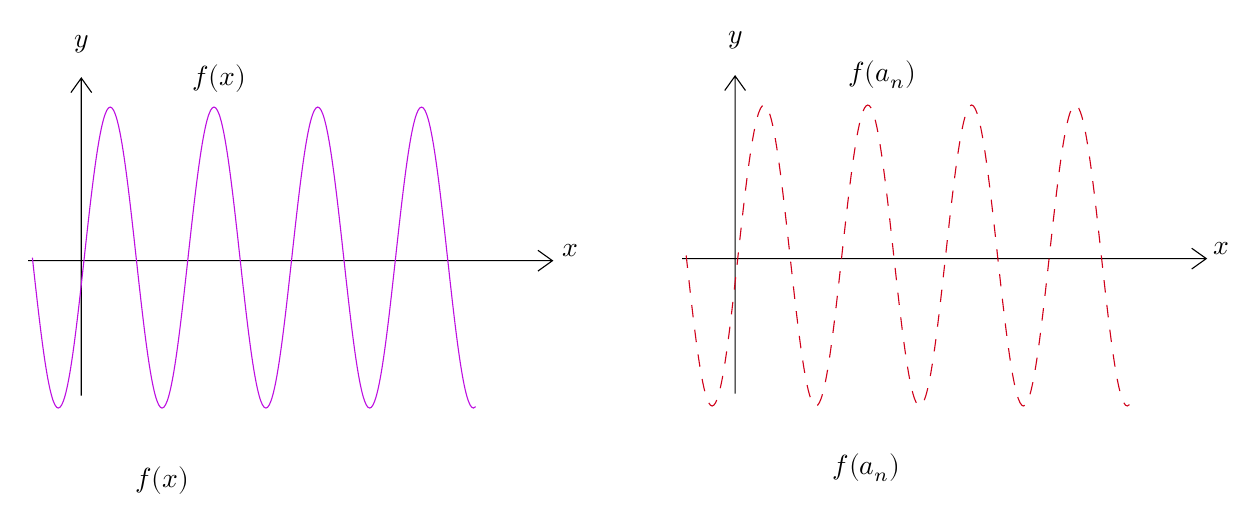
\begin{tikzpicture}[x=0.75pt,y=0.75pt,yscale=-1,xscale=1]
%uncomment if require: \path (0,300); %set diagram left start at 0, and has height of 300
%Shape: Axis 2D [id:dp017003131307001818] 
\draw  (57,165) -- (309.57,165)(82.57,77) -- (82.57,230) (302.57,160) -- (309.57,165) -- (302.57,170) (77.57,84) -- (82.57,77) -- (87.57,84)  ;
%Shape: Wave [id:dp30207647780524005] 
\draw  [color={rgb, 255:red, 189; green, 16; blue, 224 }  ,draw opacity=1 ] (59,163.5) .. controls (63.08,200.64) and (66.98,236) .. (71.5,236) .. controls (76.02,236) and (79.92,200.64) .. (84,163.5) .. controls (88.08,126.36) and (91.98,91) .. (96.5,91) .. controls (101.02,91) and (104.92,126.36) .. (109,163.5) .. controls (113.08,200.64) and (116.98,236) .. (121.5,236) .. controls (126.02,236) and (129.92,200.64) .. (134,163.5) .. controls (138.08,126.36) and (141.98,91) .. (146.5,91) .. controls (151.02,91) and (154.92,126.36) .. (159,163.5) .. controls (163.08,200.64) and (166.98,236) .. (171.5,236) .. controls (176.02,236) and (179.92,200.64) .. (184,163.5) .. controls (188.08,126.36) and (191.98,91) .. (196.5,91) .. controls (201.02,91) and (204.92,126.36) .. (209,163.5) .. controls (213.08,200.64) and (216.98,236) .. (221.5,236) .. controls (226.02,236) and (229.92,200.64) .. (234,163.5) .. controls (238.08,126.36) and (241.98,91) .. (246.5,91) .. controls (251.02,91) and (254.92,126.36) .. (259,163.5) .. controls (263.08,200.64) and (266.98,236) .. (271.5,236) .. controls (271.86,236) and (272.22,235.77) .. (272.57,235.34) ;
%Shape: Axis 2D [id:dp3577874261347358] 
\draw  (372,164) -- (624.57,164)(397.57,76) -- (397.57,229) (617.57,159) -- (624.57,164) -- (617.57,169) (392.57,83) -- (397.57,76) -- (402.57,83)  ;
%Shape: Wave [id:dp5769071550363087] 
\draw  [color={rgb, 255:red, 208; green, 2; blue, 27 }  ,draw opacity=1 ][dash pattern={on 4.5pt off 4.5pt}] (374,162.5) .. controls (378.08,199.64) and (381.98,235) .. (386.5,235) .. controls (391.02,235) and (394.92,199.64) .. (399,162.5) .. controls (403.08,125.36) and (406.98,90) .. (411.5,90) .. controls (416.02,90) and (419.92,125.36) .. (424,162.5) .. controls (428.08,199.64) and (431.98,235) .. (436.5,235) .. controls (441.02,235) and (444.92,199.64) .. (449,162.5) .. controls (453.08,125.36) and (456.98,90) .. (461.5,90) .. controls (466.02,90) and (469.92,125.36) .. (474,162.5) .. controls (478.08,199.64) and (481.98,235) .. (486.5,235) .. controls (491.02,235) and (494.92,199.64) .. (499,162.5) .. controls (503.08,125.36) and (506.98,90) .. (511.5,90) .. controls (516.02,90) and (519.92,125.36) .. (524,162.5) .. controls (528.08,199.64) and (531.98,235) .. (536.5,235) .. controls (541.02,235) and (544.92,199.64) .. (549,162.5) .. controls (553.08,125.36) and (556.98,90) .. (561.5,90) .. controls (566.02,90) and (569.92,125.36) .. (574,162.5) .. controls (578.08,199.64) and (581.98,235) .. (586.5,235) .. controls (586.86,235) and (587.22,234.77) .. (587.57,234.34) ;
\draw (78,55) node [anchor=north west][inner sep=0.75pt]   [align=left] {$\displaystyle y$};
\draw (393,53) node [anchor=north west][inner sep=0.75pt]   [align=left] {$\displaystyle y$};
\draw (313,156) node [anchor=north west][inner sep=0.75pt]   [align=left] {$\displaystyle x$};
\draw (627,155) node [anchor=north west][inner sep=0.75pt]   [align=left] {$\displaystyle x$};
\draw (100,263) node [anchor=north west][inner sep=0.75pt]   [align=left] {函数$\displaystyle f( x) 图像$};
\draw (135,69.4) node [anchor=north west][inner sep=0.75pt]    {$f( x)$};
\draw (451,67.4) node [anchor=north west][inner sep=0.75pt]    {$f( a_{n})$};
\draw (436,257) node [anchor=north west][inner sep=0.75pt]   [align=left] {函数$\displaystyle f( a_{n}) 图像$};
\end{tikzpicture}
\end{center}
    \textcolor{red}{如上图所示$f(a_n)$其实是$f(x)$的抽样}
    \begin{center}
        \tikzset{every picture/.style={line width=0.75pt}} %set default line width to 0.75pt       
        \begin{tikzpicture}[x=0.75pt,y=0.75pt,yscale=-1,xscale=1]
        \draw  [color={rgb, 255:red, 189; green, 16; blue, 224 }  ,draw opacity=1 ] (59,163.5) .. controls (63.08,200.64) and (66.98,236) .. (71.5,236) .. controls (76.02,236) and (79.92,200.64) .. (84,163.5) .. controls (88.08,126.36) and (91.98,91) .. (96.5,91) .. controls (101.02,91) and (104.92,126.36) .. (109,163.5) .. controls (113.08,200.64) and (116.98,236) .. (121.5,236) .. controls (126.02,236) and (129.92,200.64) .. (134,163.5) .. controls (138.08,126.36) and (141.98,91) .. (146.5,91) .. controls (151.02,91) and (154.92,126.36) .. (159,163.5) .. controls (163.08,200.64) and (166.98,236) .. (171.5,236) .. controls (176.02,236) and (179.92,200.64) .. (184,163.5) .. controls (188.08,126.36) and (191.98,91) .. (196.5,91) .. controls (201.02,91) and (204.92,126.36) .. (209,163.5) .. controls (213.08,200.64) and (216.98,236) .. (221.5,236) .. controls (226.02,236) and (229.92,200.64) .. (234,163.5) .. controls (238.08,126.36) and (241.98,91) .. (246.5,91) .. controls (251.02,91) and (254.92,126.36) .. (259,163.5) .. controls (263.08,200.64) and (266.98,236) .. (271.5,236) .. controls (271.86,236) and (272.22,235.77) .. (272.57,235.34) ;
        %Shape: Wave [id:dp5769071550363087] 
        \draw  [color={rgb, 255:red, 208; green, 2; blue, 27 }  ,draw opacity=1 ][dash pattern={on 4.5pt off 4.5pt}] (374,162.5) .. controls (378.08,199.64) and (381.98,235) .. (386.5,235) .. controls (391.02,235) and (394.92,199.64) .. (399,162.5) .. controls (403.08,125.36) and (406.98,90) .. (411.5,90) .. controls (416.02,90) and (419.92,125.36) .. (424,162.5) .. controls (428.08,199.64) and (431.98,235) .. (436.5,235) .. controls (441.02,235) and (444.92,199.64) .. (449,162.5) .. controls (453.08,125.36) and (456.98,90) .. (461.5,90) .. controls (466.02,90) and (469.92,125.36) .. (474,162.5) .. controls (478.08,199.64) and (481.98,235) .. (486.5,235) .. controls (491.02,235) and (494.92,199.64) .. (499,162.5) .. controls (503.08,125.36) and (506.98,90) .. (511.5,90) .. controls (516.02,90) and (519.92,125.36) .. (524,162.5) .. controls (528.08,199.64) and (531.98,235) .. (536.5,235) .. controls (541.02,235) and (544.92,199.64) .. (549,162.5) .. controls (553.08,125.36) and (556.98,90) .. (561.5,90) .. controls (566.02,90) and (569.92,125.36) .. (574,162.5) .. controls (578.08,199.64) and (581.98,235) .. (586.5,235) .. controls (586.86,235) and (587.22,234.77) .. (587.57,234.34) ;
        % Text Node
        \draw (135,69.4) node [anchor=north west][inner sep=0.75pt]    {$f( x)$};
        % Text Node
        \draw (451,67.4) node [anchor=north west][inner sep=0.75pt]    {$f( a_{n})$};
        % Text Node
        \draw (88,247) node [anchor=north west][inner sep=0.75pt]   [align=left] {用$\displaystyle \upvarepsilon -\delta $求它的极限};
        % Text Node
        \draw (396,252) node [anchor=north west][inner sep=0.75pt]   [align=left] {用海涅定理求它的极限};
        \end{tikzpicture}        
    \end{center}
    需要注意的是,是所有的数列(抽样)才能完全代表整体.不能说我选了某个数列有极限就代表函数有极限.

    总结:\textcolor{red}{海涅定理表述了离散与连续、数列极限与函数极限的关系.}
    \section{无穷小与无穷大}
    \subsection{无穷小}
    \begin{defn}{无穷小的定义}{}
        如果函数$f(x)$当$x\to x_0$(或 $x\to\infty$)时的极限为零,那么称函数$f(x)$为当$x\to x_0$(或$x\to\infty$)时的无穷小.
    \end{defn}
    \textbf{$f(x)$是可以本身为$0$或者无限趋近于零,其中$0$可以作为无穷小唯一常数}.
    \begin{criterion}{无穷小与函数极限的关系(脱帽法)}{}
        $\lim_{x\to\bullet}f(x)=A\Leftrightarrow f(x)=A+\alpha$,其中$\lim_{x\to\bullet}f(x)$为超实数值,其实数部分为$A$,函数$f(x)$的函数值为$A+\alpha$
    \end{criterion}
    \subsection{\textcolor{red}{无穷小的性质}}
    \begin{itemize}
        \item[1] 有限个无穷小的和是无穷小\footnote{无穷个无穷小的和不一定是无穷小,如$\lim_{n \to \infty}=(\frac{1}{n+1}+\frac{1}{n+2}+\frac{1}{n+3}\dots +\frac{1}{n+n})=\ln 2$}
            \begin{proof}
                设$\alpha_1$和$\alpha_2$为无穷小量。则$0 \leqslant |\alpha_1+\alpha_2|\leqslant |\alpha_1|+|\alpha_2|$,$|\alpha_1|+|\alpha_2|$的极限为0。证明完毕。
            \end{proof}
        \item[2] 有界函数与无穷小的乘积是无穷小\footnote{无界函数$\times$无穷小量不一定是无穷小,如$\lim_{x \to \infty}x \times \frac{1}{x}=1$}
            \begin{proof}
                $|\alpha _1|\leqslant M$,$\alpha_2$是无穷小量。那么$0\leqslant|\alpha_1 \times \alpha_2|=|\alpha_1|\times |\alpha_2|\leqslant M \times |\alpha_2|$证明完毕。
            \end{proof}
        \item[3] 有限个无穷小的乘积是无穷小\footnote{这个地方虽然张宇老师给出了证明,但是好像存在一定的争议性}
    \end{itemize}
    \subsection{\textcolor{red}{无穷小的比阶}}
    \begin{defn}{}{}
        \begin{itemize}
            \item 如果 $\lim \frac{\beta}{\alpha} =0$,那么就说 $\beta$是比$\alpha$高阶的无穷小,记作 $\beta=o(\alpha);$
            \item  如果 $\lim \frac\beta\alpha  =\infty$,那么就说 $\beta$是比 $\alpha$低阶的无穷小;
            \item 如果$\lim\frac{\beta}{\alpha} =c\neq 0$,那么就说 $\beta$ 与 $\alpha$ 是同阶无穷小 ;
            \item 如果$\lim\frac{\beta}{\alpha^{^k}} =c \neq 0$,$k > 0$,那么就说 $\beta$是关于 $\alpha$的$k$阶无穷小\footnote{不是相等,超实数系下没有加减运算,只可以进行替换运算};
            \item 如果 $\lim \frac\beta\alpha = 1$,那么就说 $\beta$ 与 $\alpha$ 是等价无穷小,记作 $\alpha\sim\beta$
        \end{itemize}
    \end{defn}
    前三个定义解释:$\lim \frac{\beta}{\alpha} =0$是指分子趋于$0$的速度比分母快,$\lim \frac\beta\alpha  =\infty$是指分子趋于$0$的速度比分母慢,$\lim\frac{\beta}{\alpha} =c\neq 0$是指趋于$0$的速度一样.

    同时需要注意的是,\textbf{并不是任意两个无穷小都可进行比阶的}.例如,当 $x\to 0$ 时,$x\sin\frac1x$与$x^2$虽然都是无穷小,但是却不可以比阶,也就是说既无高低阶之分,也无同阶可言,因为$\lim_{x \to 0}\frac{x \sin \frac{1}{x}}{x^2}=\lim_{x\to0}\frac1x\sin\frac1x$不存在,其值为$\infty$和$0$。
    \subsection{无穷小的运算}\footnote{此处多用于泰勒公式的应用中,会对上述高阶无穷小的运算提出要求}
    设$m,n$为无穷小,则
    \begin{itemize}
        \item[1.] $o(x^{m})\pm o(x^{n})=o(x^{l}),l=\min\{m,n\}$
        \item[2.] $o(x^{m})\bullet o(x^{n})=o(x^{m+n}),x^{m}\bullet o(x^{n})=o(x^{m+n})$
        \item[3.] $o(x^{m})=o(kx^{m})=k\bullet o(x^{m}),k \neq 0$
    \end{itemize}
    \subsection{无穷大}
    \begin{defn}{无穷大的定义}{}
        设函数$f(x)$在$x_0$的某一去心邻域内有定义(或$|x|$大于来一正数时有定义).如果对于任意给定的正数$M$(不论它多么大),总存在正数$\delta$(或数$X$),只要$x$适合不等式$0<|x-x_0|<\delta$(或$|x|>X$),对应的函数值$f(x)$总满足不等式
        $$
            |f(x)|>M
        $$
        那么称函数$f(x)$是当$x\to x_0$(或$x\to\infty$\footnote{等价于$x \to -\infty$同时$x \to +\infty$})时的无穷大.\footnote{\textbf{无穷大一定无界,但无界不一定是无穷大量。}与无穷小相同,都是一个极限过程,因此无穷大也是一个极限,所以无界不一定是无穷大量}
        其$\varepsilon-N$语言为
        $$
            \lim\limits_{x\to x_0}f(x)= \infty \Leftrightarrow\forall M >0,\exists\delta>0,\text{当}0<|x-x_0|<\delta\text{时},\text{有}|f(x)|>M.
        $$
    \end{defn}
    \begin{problem}
    证明$\underset{x\rightarrow1}{\operatorname*{lim}}\frac{1}{x-1}=\infty $
    \end{problem}
    \begin{solution}
        $\forall M>0$令$\delta=\frac{1}{4M}>0$,当$0<|x-1|<\delta$时,即$0<|x-1|<\frac{1}{4M}$时,$|x-1|<\frac{1}{M}$,所以$\frac{1}{|x-1|}>M$
        这就证明了$\underset{x\rightarrow1}{\operatorname*{lim}}\frac{1}{x-1}=\infty$
    \end{solution}
    \begin{criterion}{无穷大与无穷小的关系}{}
        在自变量的同一变化过程中,如果$f(x)$为无穷大,那么$\frac{1}{f(x)}$为无穷小;反之,如果$f(x)$为无穷小,且$f(x) \neq 0$,那么存在常数$\frac{1}{f(x)}为无穷大$
    \end{criterion}
    \subsection{\textcolor{red}{无穷大的比阶}}
    \begin{itemize}
        \item 当$x \to +\infty$时,$\mathrm{ln}^ax\ll x^\beta\ll a^x,\text{其中}\alpha>0,\beta>0,a>1.$\footnote{由洛必达公式证明}
        \item 当$n \to \infty$时,$\ln^an\ll n^\beta\ll a^n\ll n!\ll n^n,\text{其中 }\alpha>0,\beta>0,a>1.$
    \end{itemize}
    \subsection{\textcolor{red}{无穷大的性质}}
    \begin{itemize}
        \item 两个无穷大量的积仍未无穷大量
        \item 无穷大量与有界变量的和仍是无穷大量
    \end{itemize}
    \section{函数极限的运算}
    \subsection{极限的四则运算法则}
    如果极限不存在,那么极限属于超实数系的范畴,在超实数系下不可以进行代数运算,只可以进行替换运算。但是如果极限均存在,那么可以进行代数计算。\\
    若$\lim f(x)=A$,$\lim g(x)=B$,那么
    \begin{itemize}
        \item $\operatorname*{lim}[kf(x)\pm lg(x)]=k\operatorname*{lim}f(x)\pm l\operatorname*{lim}g(x)=kA\pm lB$,其中$k,l$为常数
        \item $\operatorname*{lim}[f(x)\bullet g(x)]=\operatorname*{lim}f(x)\bullet\operatorname*{lim}g(x)\equiv A\bullet B$,特别的,若$\lim f(x)$存在,$n$为正整数,则$\operatorname{lim}[f(x)]^n=\begin{bmatrix}\operatorname{lim}f(x)\end{bmatrix}^n$
        \item $\operatorname*{lim}\frac{f(x)}{g(x)}=\frac{\operatorname*{lim}f(x)}{\operatorname*{lim}g(x)}=\frac{A}{B}(B\neq0)$
    \end{itemize}
    \begin{criterion}{常用结论}{}
        \begin{itemize}
            \item 存在 \pm 不存在 = 不存在(只有这一个是不存在,其余都是不一定或者存在)
            \item 不存在 \pm 不存在 =不一定\footnote{反例:$\lim _{x \to 0}(\sin \frac{1}{x}-\sin \frac{1}{x})=0$}
            \item 存在 \times (\div) 不存在 = 不一定
            \item 不存在 \times (\div) 不存在 = 不一定
            \item 若$\lim f(x) = A \neq 0$,则$\lim f(x)\lim g(x)=A \times \lim g(x)$
        \end{itemize}
    \end{criterion}
    \begin{problem}
    \textbf{若$\lim \frac{f(x)}{g(x)}=A \neq 0$,则$\lim f(x)=0 ,\lim g(x)=0 $}
    \end{problem}
    \begin{proof}
        $g(x)=\frac{f(x)}{\frac{f(x)}{g(x)}}$。求极限得$\lim g(x)=\lim \frac{f(x)}{\frac{f(x)}{g(x)}}=\frac{\lim f(x)}{\lim \frac{f(x)}{g(x)}}=0$.证明完毕\footnote{此证明为结论,经常使用}。
    \end{proof}
    \subsection{洛必达法则}
    \begin{defn}{}{}
        \begin{itemize}
            \item $\lim_{x\to x_0}f(x)=\lim_{x\to x_0}g(x)=0(\infty)$
            \item $f(x)$和$g(x)$在$x_0$的某去心邻域内可导,且$g'(x) \neq 0$
            \item $\lim_{x\to x_0}\frac{f^{\prime}(x)}{g^{\prime}(x)}\text{ 存在(或 }\infty)$
        \end{itemize}
        则$\lim_{x\to x_{0}}\frac{f(x)}{g(x)}=\lim_{x\to x_{0}}\frac{f^{'}(x)}{g^{'}(x)}$
    \end{defn}
    \textbf{需要注意的是使用过洛必达法则之后的极限必须存在,即$\lim _{x \to x_0}\frac{f'(x)}{g'(x)}$ 必须存在.}
    \begin{problem}
    求$\lim _{x \to 0}\frac{x^2 \times \sin \frac{1}{x}}{\sin x}$
    \end{problem}
    \begin{solution}
        该函数也是$\frac{0}{0}$型,但是如果使用洛必达法则,则$2x \times \sin \frac{1}{x}-\cos \frac{1}{x}$,极限显然不存在,因此不可以使用洛必达法则。则正确求法为$\lim _{x\to 0}\frac{x^2\times \sin \frac{1}{x}}{x}=\lim_{x\to 0}x\times\sin\frac{1}{x}=0$.
    \end{solution}
    \subsection{泰勒公式}
    设$f(x)$在点$x=0$处$n$阶可导\footnote{泰勒公式是在一点处展开,函数必须在那一点处n阶导数存在},则存在$x=0$的一个邻域,对于该领域内的任一点$x$,有:
    $$
        f(x)=f(0)+f'(0)x+\frac{f''(0)}{2!}x^2+\cdots+\frac{f^{(n)}(0)}{n!}x^n+o(x^n)
    $$
    当$x\to 0$时,有以下结论
    \begin{align*}
        \boxed{\begin{aligned}
                        & \sin x =x-\frac{x^3}{3!}+o(x^3)                                &  & \cos x =1-\frac{x^2}{2!}+\frac{x^4}{4!}+o(x^4)                  \\
                        & \arcsin x =x+\frac{x^3}{3!}+o(x^3)                             &  & \tan x =x+\frac{x^3}3+o(x^3)                                    \\
                        & \arctan x =x-\frac{x^{3}}{3}+o(x^{3})                          &  & \ln(1+x) =x-\frac{x^{2}}{2}+\frac{x^{3}}{3}+o(x^{3})            \\
                        & \mathrm{e}^{x} =1+x+\frac{x^{2}}{2!}+\frac{x^{3}}{3!}+o(x^{3}) &  & (1+x)^{a} =1+\alpha x+\frac{\alpha(\alpha-1)}{2!}x^{2}+o(x^{2}) \\
                   \end{aligned}}
    \end{align*}
    \begin{criterion}{泰勒公式应用时的展开原则}{}
        \begin{itemize}
            \item $\frac{A}{B}$型,适用于"上下同阶"原则:具体来说,如果分母或者分子是$x$的$k$次幂,则应把分子或分母展开到$x$的$k$次幂。如:$\lim_{x\to0}\frac{x-\ln(1+x)}{x^{2}}$,此处$\ln(1+x)$应展开为$x-\frac{x^2}{2}+o(x^2)$
            \item $A-B$型,适用"幂次最低"原则:将$A,B$分别展开到他们系数不相等的$x$的最低次幂为止。如:已知当$x\to0$时,$\cos x-e^{\frac{x^2}2}$与$ax^b$为等价无穷小,求$a,b$.则应展开为$\cos x=1-\frac{x^2}{2!}+\frac{x^4}{4!}+o(x^4),\mathrm{e}^{-\frac{x^2}{2}}=1-\frac{x^2}{2}+\frac{1}{2!}\frac{x^4}{4}+o(x^4).$
        \end{itemize}
    \end{criterion}
    \subsection{极限存在准则的两个应用(两个重要极限)}
    $$
        \lim _ { \square \rightarrow \infty } ( 1 + \frac { 1 } { \square } ) ^ { \square } = e
    $$
    \\
    $$
        \lim _ { \square \rightarrow 0 } \frac { \sin \square } { \square } = 1
    $$

    \subsection{夹逼准则}
    \begin{defn}{函数极限存在准则}{}
        如果
        \begin{itemize}
            \item 当$x\in U^{\circ}(x_{0},r)($ 或 $|x|>M)$ 时
                  $$
                      g(x)\leqslant f(x) \leqslant h(x)
                  $$
            \item $\lim_{x\to x_0(x\to\infty)}g(x)=A,\lim_{x\to x_0(x\to\infty)}h(x)=A$
        \end{itemize}
        那么$\lim_{x\to x_0(x\to\infty)}f(x)$存在,且等于$A$.
    \end{defn}
    \begin{itemize}
        \item 夹逼准则处主要通过放缩来求极限
        \item 常用的结论有:若$\lim _{n \to \infty} \sqrt[n]{a_1^n+a_2^n+...+a_m^n}$,其中$a_i >0(i=1,2,3,...,m)$,令$\max{a_i}=a$,则$\sqrt[n]{a^n}\leqslant\sqrt[n]{a_1^n+a_2^n+\cdots+a_m^n}\leqslant\sqrt[n]{ma^n}$,\\$\lim_{n\to\infty}\sqrt[n]{a^n}=a,\lim_{n\to\infty}\sqrt[n]{m\cdot a^n}=a$,则$\operatorname*{lim}_{n\to\infty}\sqrt[n]{a_1^n+a_2^n+\cdots+a_m^n}=a$
    \end{itemize}
    \subsection{\textcolor{red}{单调有界准则}}
    \begin{defn}{函数的单调有界准则}{}
        设函数$f(x)$在点$x_0$的某个左邻域内单调并且有界,则$f(x)$在$x_0$的左极限$f(x_0^-)$一定存在
    \end{defn}

    \subsection{函数极限的运算法则}
    \begin{defn}{}{}
        如果$\varphi(x)\geqslant\psi(x)$,而 $\lim\varphi(x)=A$, $lim \psi(x)=B$ ,那么 $A\geqslant B$
    \end{defn}
    \begin{defn}{复合函数极限运算法则}{}
        设函数$y=f[g(x)]$是由函数$u=g(x)$与函数$y=f(u)$复合而成,$f[g(x)]$在点$x_0$的某去心领域内有定义,若$\lim_{x \to  x_0} g(x)=u_0$,$\lim_{u \to u_0}f(u)=A$,且存在$\delta_0 >0$,当$x\in\mathring{U}\left(x_{0},\delta_{0}\right)$时,有$g\left(x\right)\neq u_{0}$,则
        $$
            \underset{x\to x_0}{\operatorname*{lim}}f[g(x)]=\underset{u\to u_0}{\operatorname*{lim}}f(u)=A.
        $$
    \end{defn}
    \begin{criterion}{常用的结论}{}
        \begin{itemize}
            \item $\lim f(x)=A \neq 0 \Rightarrow \lim f(x)g(x)=A \lim g(x)$
            \item $\lim \frac{f(x)}{g(x)}$存在,$\lim g(x)=0 \Rightarrow \lim f(x)=0$
        \end{itemize}
    \end{criterion}
    \subsection{等价无穷小替代}
    关于等价无穷小,有以下两个定理
    \begin{defn}{}{}
        $\beta$与$\alpha$是等价无穷小的充分必要条件为
        $$
            \beta=\alpha + o(\alpha)
        $$
    \end{defn}

    \begin{defn}{}{}
        设$\alpha\sim\widetilde{\alpha}$,$\beta\sim\widetilde{\beta}$,且$\lim\frac{\widetilde{\beta}}{\underset{\alpha}{\operatorname*{\sim}}}$存在,则
        $$
            \lim\frac{\beta}{\alpha}=\lim\frac{\widetilde{\beta}}{\overset{\sim}{\alpha}}.Í
        $$
        求两个无穷小之比的极限时,分子及分母都可用等价无穷小来代替.但是需要遵循以下代换原则\footnote{其实没有什么替换原则,本质其实是因为超实数系下不能进行实数运算,只能进行替换运算}
        \begin{itemize}
            \item 乘除关系可以换:若$\alpha\sim\alpha_1,\beta\sim\beta_1,\text{则}\lim\frac\alpha\beta=\lim\frac{\alpha_1}\beta=\lim\frac\alpha{\beta_1}=\lim\frac{\alpha_1}{\beta_1}$
            \item 加减关系一定条件下可以换
                  \begin{itemize}
                      \item 若$\alpha\sim\alpha_{1},\beta\sim\beta_{1},\text{且}\operatorname*{lim}\frac{\alpha_{1}}{\beta_{1}}=A\neq1,\text{则 }\alpha-\beta\sim\alpha_{1}-\beta_{1}$
                      \item 若$\alpha\sim\alpha_{1},\beta\sim\beta_{1},\text{且}\operatorname*{lim}\frac{\alpha_{1}}{\beta_{1}}=A\neq-1,\text{则 }\alpha+\beta\sim\alpha_{1}+\beta_{1}$
                  \end{itemize}
        \end{itemize}
        加减关系代换准则证明如下:
        \begin{proof}
            $$\lim \frac{\alpha-\beta}{\alpha_1 -\beta_1}=\lim \frac{\beta (\frac{\alpha}{\beta}-1)}{\beta_1(\frac{\alpha_1}{\beta_1}-1)}=1$$
        \end{proof}
    \end{defn}
    以下为常用等价无穷小
    \\当$x \to 0$时,有
    \begin{align*} \boxed{
            \begin{aligned}
                 & x \sim \sin x \sim \tan x \sim \arcsin x \sim \arctan x \nonumber \\
                 & \quad  \sim \ln (1+x)  \nonumber                                  \\
                 & \quad \sim e^x -1 \nonumber
            \end{aligned} }
    \end{align*}

    \begin{align*} \boxed
        {
            \begin{aligned}
                 & (1+x)^a \sim  1+ax   \\
                 & a^x - 1 \sim x \ln a
            \end{aligned}
        }
    \end{align*}
    \begin{criterion}{上述结论的推广}{}
        当$x \to 0$时,若$(1+x)^a -1 \sim ax$,则$\alpha (x) \to 0,\alpha(x)\beta(x) \to 0$,则
        $$
            [1+\alpha(x)]^{\beta(x)} -1 \sim \alpha(x) \beta(x)
        $$
    \end{criterion}
    \begin{align*} \boxed
        {
            \begin{aligned}
                 & \frac{1}{2} x^2 \sim 1-\cos x \sim \sec x -1 \sim x- \ln(1+x)
            \end{aligned}
        }
    \end{align*}

    \begin{align*} \boxed
        {
            \begin{aligned}
                 & \frac{1}{6} x^3 \sim x-\sin \sim \arcsin x -x
            \end{aligned}
        }
    \end{align*}
    \begin{align*} \boxed
        {
            \begin{aligned}
                 & \frac{1}{3} x^3 \sim x-\arctan x \sim \tan x-x
            \end{aligned}
        }
    \end{align*}
    \subsection{利用基本极限求极限}
    \begin{align*} \boxed
        {
            \begin{aligned}
                 & \lim_{\square \to \infty }(1+|\square|)^{\frac{1}{\square}}=e^{|\square| \frac{1}{\square}} \qquad     \lim _ { \square \rightarrow 0 } \frac { \sin \square } { \square } = 1 \\
                 & \lim_{n \to \infty }\sqrt[n]{n}=1 \qquad \lim_{n \to \infty} \sqrt[n]{a}=1(a>0)                                                                                                \\
                 & \lim_{x \to 0} \frac{a^x-1}{x}=\ln a
            \end{aligned}
        }
    \end{align*}
    \subsection{定积分求极限}
            % //TODO
    \subsection{七种未定式的计算}
            % //TODO
    \subsubsection{形如$\frac{0}{0}$,$\frac{\infty}{\infty}$,$0 \times \infty$}
    \subsubsection{形如$\infty -\infty$}
    \subsubsection{形如$\infty^0,0^0$}
    \subsubsection{形如$1^{\infty}$}
    \section{数列极限的运算}
    \subsection{数列极限的运算法则}
    设$\underset{n\to\infty}{\operatorname*{lim}}x_{n}=a,\underset{n\to\infty}{\operatorname*{lim}}y_{n}=b$,则
    \begin{itemize}
        \item $\operatorname*{lim}_{n\to\infty}(x_n\pm y_n)=a\pm b$
        \item $\lim_{n\to\infty}x_{n}y_{n}=ab$
        \item 若$b \neq 0,y_n \neq 0$,则$\lim_{n\to\infty}\frac{x_n}{y_n}=\frac{a}{b}$
    \end{itemize}
    上述运算规则可推广至有限个数列的情况
    \subsection{夹逼准则}
    \begin{them}{数列极限存在准则}{}
        如果数列$\{|x_n|\},\{y_n\}$及$\{z_n\}$满足下列条件:
        \begin{itemize}
            \item 从某项开始,即$\exists n_0 \in N_+(\text{即}n \to \infty),$当$n>n_0$时,有
                  $$
                      y_n \leqslant x_n \leqslant z_n
                  $$
            \item $\lim_{n\to\infty}y_{n}=a,\operatorname*{lim}_{n\to\infty}z_{n}=a$
        \end{itemize}
        那么数列$\{ x_n \}$的极限存在,且$\lim_{n\to\infty}x_{n}=a$
    \end{them}
    以下为放缩的常用方法
    \begin{itemize}
        \item 利用简单放大与缩小
        $$\begin{cases}n\times u_{\min}\leqslant u_1+u_2+\cdots+u_n\leqslant n\times u_{\max},\\\text{当}u_i\geqslant0\text{时,1}\times u_{\max}\leqslant u_1+u_2+\cdots+u_n\leqslant n\times u_{\max}.\end{cases}$$
        \item 利用如下重要不等式
        \begin{problem}
            $\lim\limits_{n\to\infty}\Bigg(\frac{1}{n^2+n+1}+\frac{2}{n^2+n+2}+\cdots+\frac{n}{n^2+n+n}\Bigg)$
        \end{problem}
        \begin{proof}
            
        \end{proof}
        \begin{problem}
            求极限$\lim_{n\to\infty}\sqrt[n]{a_1^n+a_2^n+\cdots+a_m^n}$,其中$a_i(i=1,2,\cdots,m)$都是非负数
        \end{problem}
        \begin{proof}
            
        \end{proof}
        \begin{enumerate}
            \item 设$a,b$为实数,则$|a+b|\leq |a|+|b|$;$\mid|a|-|b|\mid\leqslant|a-b|$\footnote{
                可以将上述式子推广为n个实数的情况:$|a_1\pm a_2\pm\cdots\pm a_n|\leqslant|a_1|+|a_2|+\cdots+|a_n|.$}
            \item $\sqrt{ab}{\leqslant}\frac{a+b}{2}{\leqslant}\sqrt{\frac{a^{2}+b^{2}}{2}}(a,b{>}0)\footnote{还有一个不等式是$|ab|\leqslant \frac{a^2+b^2}{2}$}$
            \item $\sqrt[3]{abc}\leqslant\frac{a+b+c}3\leqslant\sqrt{\frac{a^2+b^2+c^2}3}(a,b,c>0)$
            \item $\text{设 }a\geq b\geq 0,\text{则}\left\{\begin{aligned}&\text{当 }n\geq 0\text{ 时 },a^n\geq b^n,\\&\text{当 }n \leqslant 0\text{ 时 },a^n \leqslant b^n.\end{aligned}\right.$
            \item $\text{若 }0<a<x<b,0<c<y<d,\text{则}\frac{c}{b}<\frac{y}{x}<\frac{d}{a}.\footnote{$\text{当 }n\pi<x<(n+1)\pi,2n<S(x)<2(n+1)\text{时 },\frac{2n}{(n+1)\pi}<\frac{S(x)}{x}<\frac{2(n+1)}{n\pi}.$}$
            \item $\sin x<x<\tan x\left(0<x<\frac{\pi}{2}\right)$
            \item $\sin x < x(x>0)$
            \item 当$0<x<\frac{\pi}{4}$时,$x<\tan x<\frac{4}{\pi}x$
            \item 当$0<x<\frac{\pi}{2}$时,$\sin x>\frac{2}{\pi}x$
            \item $\arctan x{\leqslant}x{\leqslant}\arcsin x(0{\leqslant}x{\leqslant}1)$
            \item $e^x \geqslant  x+1 (\forall x)\footnote{  $\text{当 }x_{n+1}=\mathrm{e}^{x_n}-1\text{ 时 ,由 }\mathrm{e}^{x_n}-1\geqslant x_n,\text{得 }x_{n+1}\geqslant x_n,\text{即} \{x_n\} \text{单调不减}$}$
            \item $x-1 \geqslant \ln x(x>0)\footnote{                  $\text{当 }x_{n}>0\text{时,若 }x_{n+1}=\ln x_{n}+1,\text{由}\ln x_{n}+1\leqslant x_{n},\text{得 }x_{n+1}\leqslant x_{n},\text{即}\{ x_{n}\} \text{单调不增}$}$
            \item $\frac{1}{1+x}<\ln(1+\frac{1}{x})<\frac{1}{x}(x>0)$或 $\frac{x}{1+x}<\ln(1+x)<x(x>0)$\footnote{
                令$f(x)=\ln x$,并在区间$[x,x+1]$上对其使用拉格朗日中值定理,有$\ln\left(1+\frac{1}{x}\right)=\ln(1+x)-\ln x=\frac{1}{\xi}$其中$0<x<\xi<x+1$,因此对任意的$x>0$,有$\frac{1}{1+x}<\ln\left(1+\frac{1}{x}\right)=\frac{1}{\xi}<\frac{1}{x}$}
            \item 在处理如下数列时,可以在前面加一个减项,如$(1+\frac{1}{2^2})(1+\frac{1}{2^{2^2}})...(1+\frac{1}{2^{2^n}})$,可化为$(1-\frac{1}{4})(1+\frac{1}{2^2})(1+\frac{1}{2^{2^2}})...(1+\frac{1}{2^{2^n}})*\frac{4}{3}$
        \end{enumerate}
        \item 利用闭区间上连续函数必有最大值与最小值
        \item 利用压缩映射原理
        % //TODO
    \end{itemize}
    \subsection{\textcolor{red}{单调有界准则}}
    \begin{them}{数列的单调有界准则}{}
        单调有界数列必有极限,即若数列$\{x_n\}$单调增加(减少)且有上界(下界),则$\lim_{n \to \infty} x_n$存在
    \end{them}
    %  ############################ 正文部分
    \ifx\allfiles\undefined
\end{sloppypar}
\end{document}
\fi
